% !TEX root = BA-Bauer.tex

\subsection{Platinendesign} \label{sec:PCB-Design}
Das Design der Platine spielt eine wichtige Rolle in der Entwicklung des Gerätes, denn es müssen alle 78\,Komponenten auf ihr Platz finden, sie muss elektrisch und logisch sinnvoll aufgebaut sein und gleichzeitig kompakte Maße haben, damit das Endprodukt handlich ist. Zudem kommen einige technische Anforderung von Bauteilen, wie die Platzierung der Stützkondensatoren des MCUs, die möglichst nah an diesem platziert werden müssen, hinzu. Außerdem muss der SD-Kartensteckplatz im Nachhinein für den Benutzer zugänglich sein, der Benutzer muss die Taster betätigen, die LEDs leuchten, den LCD sehen können und in der Lage dazu sein die DMX- und das USB-Kabel in die entsprechenden Buchsen zu stecken.
\begin{figure}[h]
	\centering
	\begin{minipage}[t]{0.47\linewidth}
		\centering
		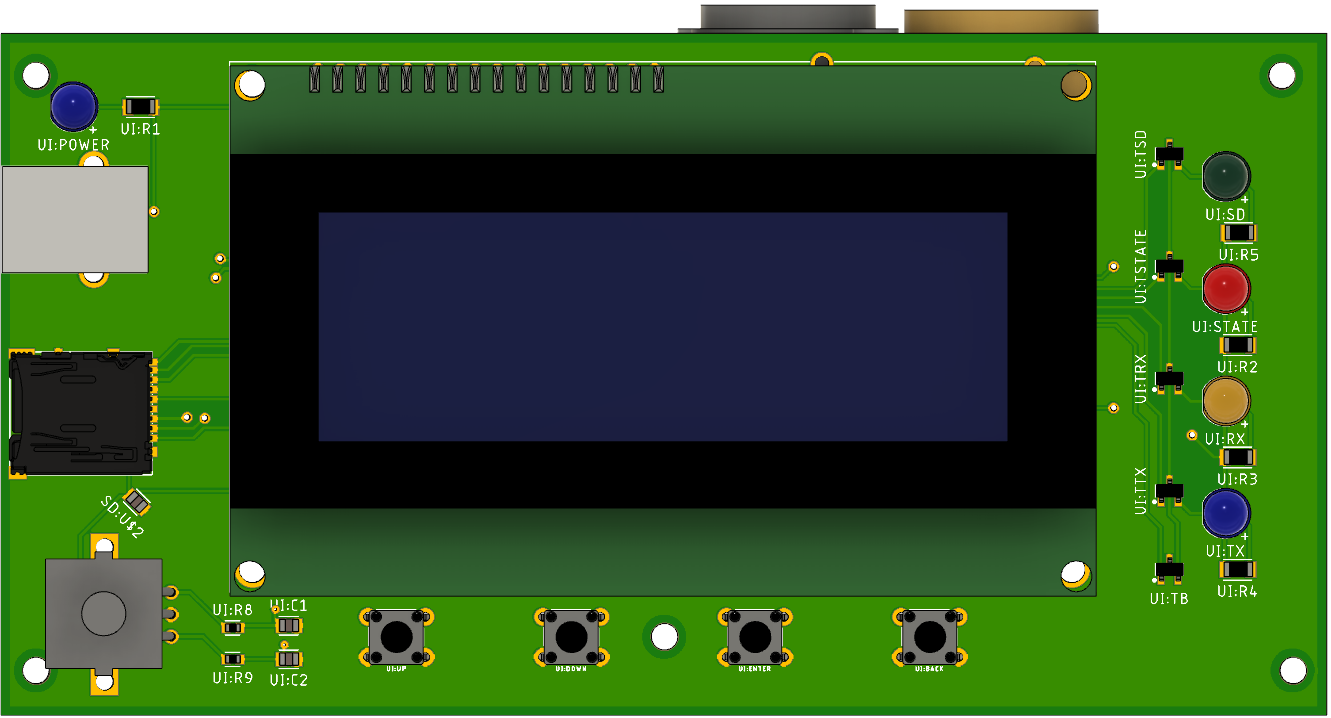
\includegraphics[width=\linewidth]{PCB_top}
		\caption{Platinenvorderseite}
		\label{fig:PCB-top}
	\end{minipage}
	\hfil
	\begin{minipage}[t]{0.47\linewidth}
		\centering
		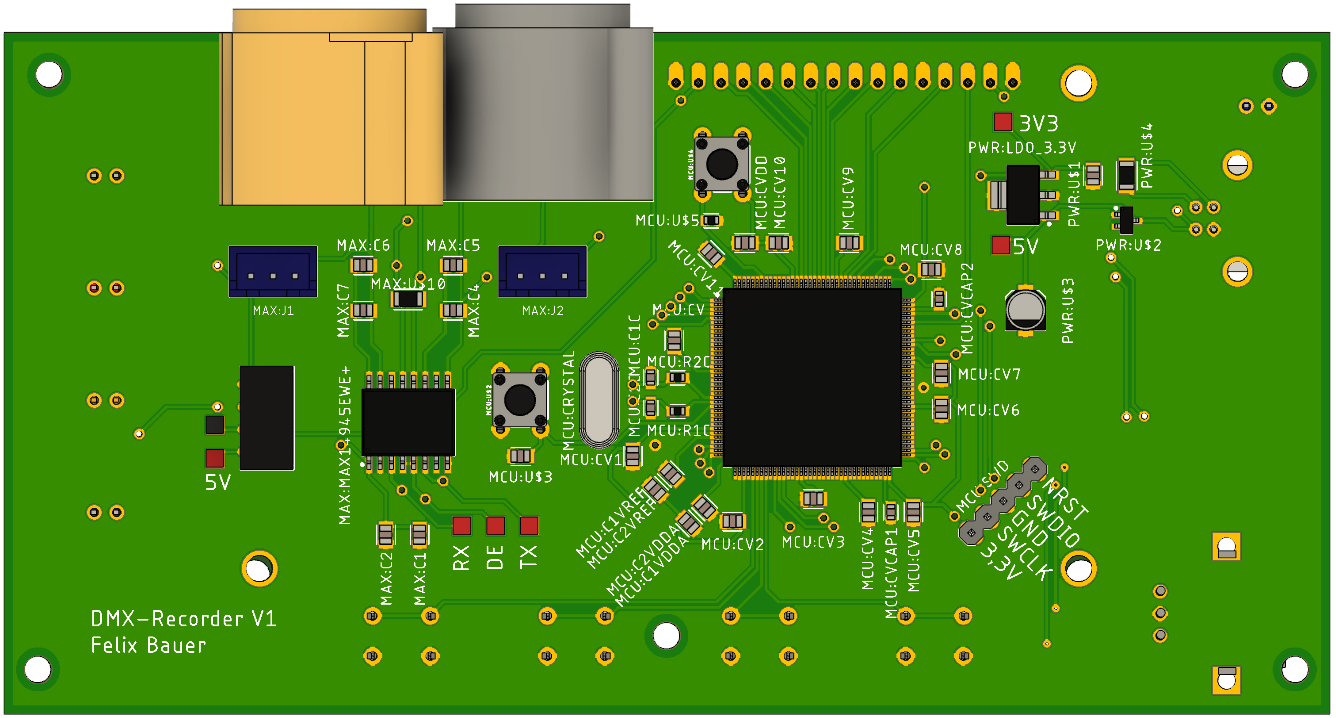
\includegraphics[width=\linewidth]{PCB_bottom}
		\caption{Platinenrückseite}
		\label{fig:PCB-bottom}
	\end{minipage}
\end{figure}\\
Abbildung \ref{fig:PCB-top} und \ref{fig:PCB-bottom} zeigen das Layout der Platine als virtuelles, dreidimensionales Modell. 
Auf der Platine werden zwei Arten von Komponenten verbaut. Zum Einen sogenannte \textit{surface-mount-technology}-Komponenten (SMT-Komponenten), zum Anderen \textit{through-hole-technology}-Komponenten (THT-Kom-ponenten). SMT-Komponenten werden direkt auf die Oberfläche der Platine gelötet, weswegen für diese keine Löcher in der Platine notwendig sind. Durch die Oberflächenmontage befindet sich das Bauteil auf der selben Seite wie die dazugehörige Lötstelle. Für THT-Komponenten werden Löcher in der Platine benötigt, da die Pins der Komponenten im 90\,$^\circ$-Winkel zur Oberfläche der Platine stehen. Diese können unter Umständen nur auf der gegenüberliegenden Seite der Platine verlötet werden. Eine LED zum Beispiel, die bündig mit der Platine verlötet werden soll, kann nur auf der gegenüberliegenden Seite der Platine verlötet werden, da die LED selbst ihre eigenen Pins verdeckt. Damit alle Komponenten frei auf der Platine platziert werden können, wird eine zweiseitige Platine entworfen. Diese besitzt auf der Vorder- und Rückseite je eine Kupferschicht, welche mithilfe von sogenannten \textit{Vias}\footnote{Durchkontaktierte Löcher in der Platine} verbunden werden können.
\begin{figure}[h]
	\begin{center}
		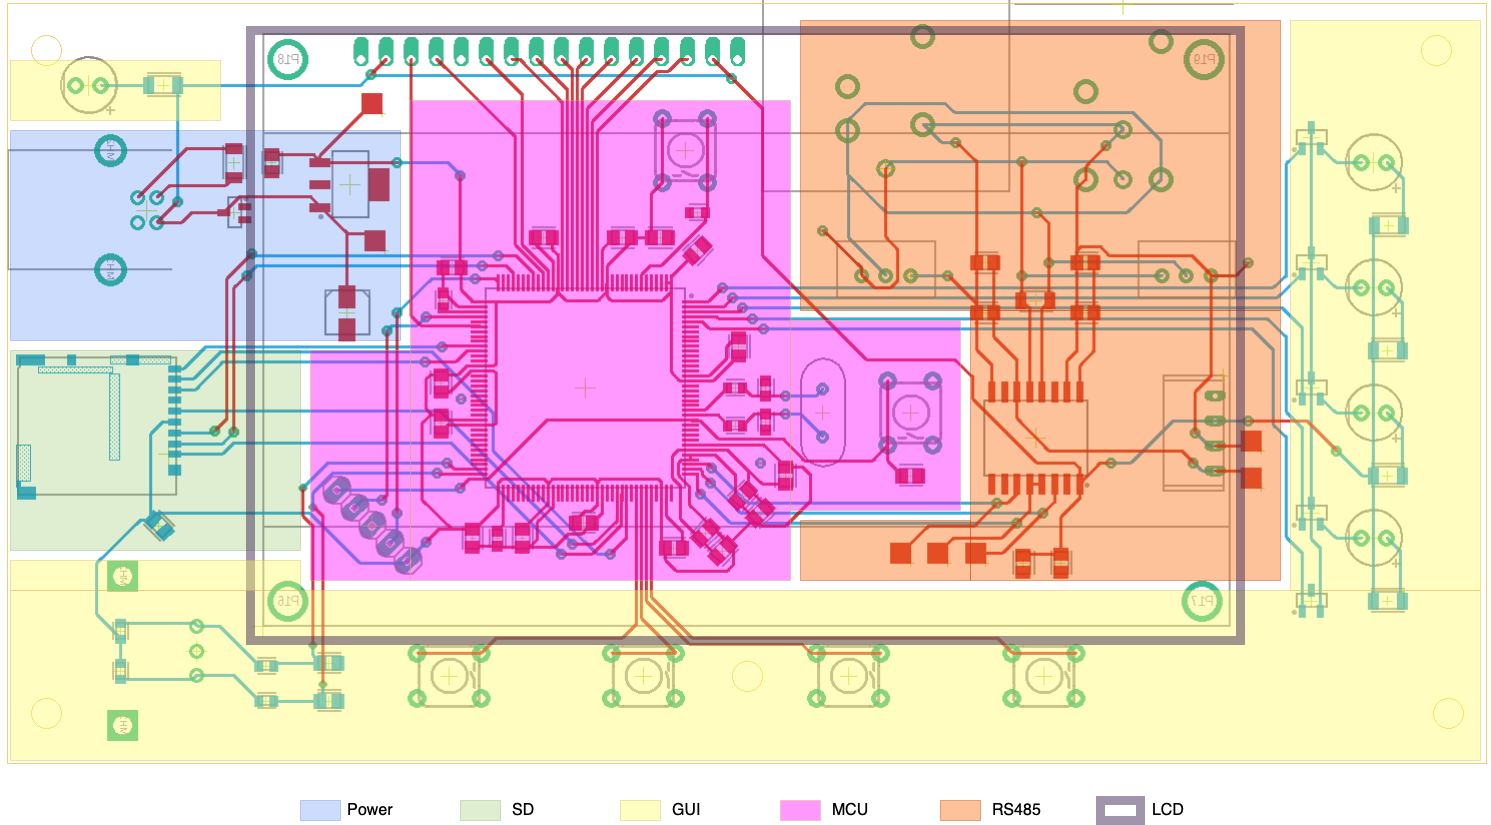
\includegraphics[width=\linewidth]{PCB-Design_mark}
		\caption{Platinenlayout-Aufteilung}
		\label{fig:PCB-Layout}
	\end{center}
\end{figure}
Abbildung \ref{fig:PCB-Layout} zeigt die generelle Aufteilung der Platine. Diese Aufteilung vereinfacht die mögliche Fehlersuche und trägt dazu bei die Leiterbahnlängen zu verkürzen. Alle blau gefärbten $Pads$\footnote{In der Regel rechteckige Lötstellen (freigelegte Kupferflächen) zum verlöten von SMT-Komponenten} und Leiterbahnen befinden sich auf der Vorderseite, alle rot eingefärbten auf der Rückseite der Platine. Die freien Flächen zwischen den Leiterbahnen auf der Ober- und Unterseite sind mit dem 0\,V Potential verbunden. Die grünen Bohrungen sind $Vias$ und durchkontaktierte Bohrungen für die THT-Komponenten.
Der Formfaktor der Platine wird im Wesentlichen von dem LCD-Modul vorgegeben, da es das größte Bauteil darstellt. Neben dem LCD-Modul muss außerdem Platz für den Encoder, die Taster und LEDs vorhanden und für den Benutzer sichtbar und verwendbar sein. Aus diesem Grund werden das LCD-Modul, die Taster, der Encoder und die LEDs auf der Vorderseite der Platine platziert. Im Zentrum der Platine befindet sich das LCD-Modul. Unterhalb des Moduls befinden sich die Taster, rechts davon die LEDs. Die LED, die den Zustand der Spannungsversorgung anzeigt, befindet sich oben links um eine Verwechslungen mit der zweiten blauen LED zu verhindern. Der SD-Kartensteckplatz, grün markiert, findet am linken Rand unterhalb der USB-Buchse und Schaltung der Spannungsversorgung, blau markiert, der Platine Platz. Der MCU bildet den größten Knotenpunkt der Schaltung und befindet sich deswegen in der Mitte der Platine. Laut Hersteller sollen die Stützkondensatoren möglichst nah am MCU platziert werden, damit die Induktivität der Leiterbahnen den hohen Stromfluss aus den Kondensatoren heraus nicht beeinträchtigt, wie bereits in Kapitel \ref{sec:STM} erläutert. Kritische, an den MCU angeschlossene Komponenten sind unter anderem der SD-Kartenslot, der Quartz und der RS485-Treiberchip. Damit möglichst wenige Störungen auf die Leiterbahnen einwirken können, sind diese möglichst kurz. Die XLR-Buchsen für die ein- und ausgehenden DMX-Daten befinden sich am oberen Rand der Rückseite der Platine. Sie und die Schaltung des Treiberchips, rot markiert, liegen nah beieinander um auch hier das Störungspotential durch lange Leiterbahnen möglichst gering zu halten.